\documentclass[11pt]{article}
\usepackage{geometry}                % See geometry.pdf to learn the layout options. There are lots.
\geometry{letterpaper}                   % ... or a4paper or a5paper or ... 
%\geometry{landscape}                % Activate for for rotated page geometry
%\usepackage[parfill]{parskip}    % Activate to begin paragraphs with an empty line rather than an indent
\usepackage{graphicx}
\usepackage{amssymb}
\usepackage{epstopdf}
\usepackage{indentfirst}
\DeclareGraphicsRule{.tif}{png}{.png}{`convert #1 `dirname #1`/`basename #1 .tif`.png}

\title{Evaluating the Mobile Operating System Effectively}
\author{Edward Bramanti}
%\date{}                                           % Activate to display a given date or no date

\begin{document}
\maketitle
\begin{abstract}
\end{abstract}
\pagebreak
\section{Introduction}
In today's world, mobile operating systems are now as prevalent as personal computers. More and more, consumers are turning to smartphones and tablets to daily drive their time spent in productivity as well as entertainment. As this field has continued to develop, the consumer is given a myriad of choices between many different operating systems. Hardware and software manufacturers have arisen to provide a competitive environment. This has led to successes for user choice, as hardware and software companies square off to provide the most innovative interface.\\
\indent While this has been a great success for the consumer, it has also caused problems for firms. A series of patent wars between companies has arisen in the past few years, which has demonstrated the desire for monopoly over the market by utilizing the legal system. Paik and Zhu note that "According to this view, technology firms race to assemble patent portfolios - initially for defensive purposes in the context of a dynamic and competitive field - but then, as the industry matures, convert their shields into weapons to eliminate their competitors in pursuit of market dominance with its platform."\cite{PatentWars} This desire to achieve market independence has led many reviewers to create preconceived notions that the market is no longer innovating, but instead creating a "future-proofing" system that fights pointless legal battles to control software innovation.\\
\indent Because of this new growth in the smartphone market, reviewers are pitting operating system against operating system to help the user discover if it is the best fit for them. The question remains though: Are the journalistic and firm-based reviewers doing an accurate job of evaluating a mobile operating system? In particular, we will be taking a look at Pfeiffer Consulting's "Mobile OS User Experience Shootout" as a reference for how companies conduct evaluations of mobile operating systems today, and how focusing on certain things that connect consumers and developers together through mental process will increase reasoning and understanding behind the results collected from users.

\section{Background}
\label{background}
To provide background on how evaluations of a mobile operating system should be performed, we will look at the data from the two most important points of view: first, the developer; and then, the consumer, or end-user. Seeing how the developer analyzes the operating system versus the end-user will help to provide a bridge between the mental thought process of the two, and will provide those observing a foundation for how to approach reviewing a mobile operating system effectively.
\subsection{The Developer Perspective}
Why is the developer's perspective important to evaluating a mobile operating system? Developers are essential to any platform building its ecosystem, and a mobile operating system is no exception. In addition, understanding the developer's thought process will be invaluable to hearing the other side of the story, since some evaluations of mobile OS' occur only through the eyes of the end user (Pfeiffer's report is an example). \\
\indent So how do developers evaluate mobile operating systems, and choose which is the best to design for? Palme et al. state that there are six dimensions to how a developer decides on the best mobile operating system for them: "corporate buyer choice, consumer buyer choice, OS vendor's market growth potential, ease of implementation, security, and revenue." \cite{Palme} Specifically, ease of implementation is one factor to focus on in determining if a mobile OS is successful. Evaluators generally overlook this, because they focus on the ease of use for consumer instead of the ease of implementation for the developer. Besides, the end-user never sees the developer's thought process, right? This is a common misconception amongst reviewers of mobile OS functionality. The developer's job is to mesh his mental model of how something should work with the user's model. Interaction design itself is defined this way: "A system's designer/developer must effectively communicate his mental model of the system to the system's users through the "image" presented by that system." Therefore, if the "terms and 
conditions [of the mobile Software Development Kit(SDK)]... limit[s] the freedom of development by restricting the domain of application or variety of functionality," the ease of use for the user suffers. \cite{Palme}

\begin{figure}[h]
\begin{center}
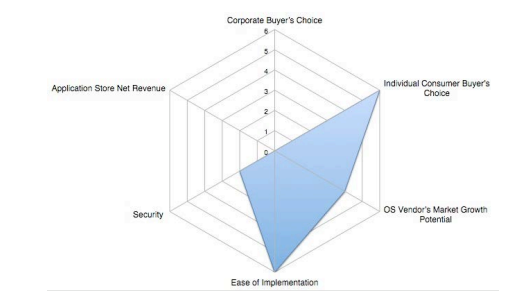
\includegraphics{developerPerspective}
\caption{This picture portrays the mental model of the developer choosing a mobile OS to design an app for. \cite{Palme}}
\label{developerPerspective}
\end{center}
\end{figure}
It is important to note the importance of the designer in the evaluation of the success of an operating system. Since the ease of implementation is heavily tied to the ease of use for the user, it would be an incomplete analysis of operating system success without considering the developer's perspective on the functionality of the OS at the software development level.

\subsection{The End-User Perspective}
When many go to evaluate and review mobile operating systems, they run unknowingly into the issue of context. During a controlled evaluation, many users may respond in a certain way to an interface. Some may respond in certain ways when placed in certain situations. But at the end of the day, what is the goal of the end-user? The end-user's experience needs to be evaluated contextually, according to Coutaz et al. The end-user value a contextual experience for their experience of an OS on the go. \cite{Coutaz} \\
\indent So, why is context a part of the end-user perspective that so many seem to gloss over? It's very difficult to gauge an experience contextually. Apps like Aviate for Android are bringing validity to the importance of contextual computing, and are showing a valid area that is being overlooked by reviewers: what users do at certain moments in certain locations. For example, Aviate considers if you are at the coffee shop by pulling your location from GPS services, and displays a new context on the launch screen with things specifically tailored to your current experience. \cite{Aviate} These kind of things matter to the end-user on a mobile operating system. Since the location of a mobile OS is not statically located like desktop operating systems, users will consider context to be essential to the experience, as can be seen in Figure \ref{aviate}. Evaluations of mobile OS' search for this key term, 

\begin{figure}[h]
\begin{center}
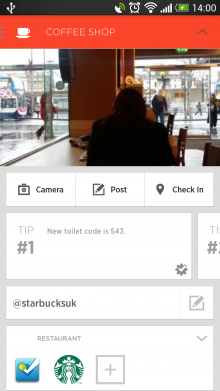
\includegraphics[height = 3in]{aviate}
\caption{Aviate is a contextual launcher application for Android. Pictured here is the mobile OS detecting the current context of the phone, and modifying its launch screen to show what the user needs in this certain situation. \cite{Aviate}}
\label{aviate}
\end{center}
\end{figure}


\section{Methods}
Now that we have filled in the background of developer and end-user perspective with past research, we can now effectively evaluate Pfeiffer Consulting's Mobile OS evaluation. Pfeiffer evaluates four "usability metrics" in a way that they describe as a "look at aspects that have a direct impact on the day-to-day user experience of an average, non-technical user." \cite{Pfeiffer} The four metrics they are analyzing will be evaluated as compared to the background found in Section \ref{background}.
\subsection{Cognitive Load Survey}
Pfeiffer takes a survey over a term they have coined "cognitive load," which "counted
the number of apps/widgets as well as other icons and user interface elements a default installation of the operating system contains." \cite{Pfeiffer} Pfeiffer uses this in their argument that the lower the cognitive load, the easier it will be for a user to navigate the operating system, at the cost of features. They define this as "the number of apps/widgets as well as other icons and user interface elements a default installation of the operating system contains." \cite{Pfeiffer} The first problem that this survey runs into, when compared to background, is how contextual computing can nullify a cognitive load test. If the end-user has an interface that is contextual (in the case of this survey, say they are using Aviate on their Samsung Android device) then the extra apps are not a hindrance, but represent a low cognitive load. The apps you need only appear based on context, which makes this survey a little difficult to quantify.
\subsection{
\section{Discussion}
\section{Conclusion}

\bibliographystyle{alpha}
\bibliography{mental-model-paper}

\end{document}  